\documentclass[tikz,border=6pt]{standalone}

\usetikzlibrary{arrows.meta,fit,positioning}

\usepackage{pgfplots}
\pgfplotsset{compat=1.18}

\begin{document}
  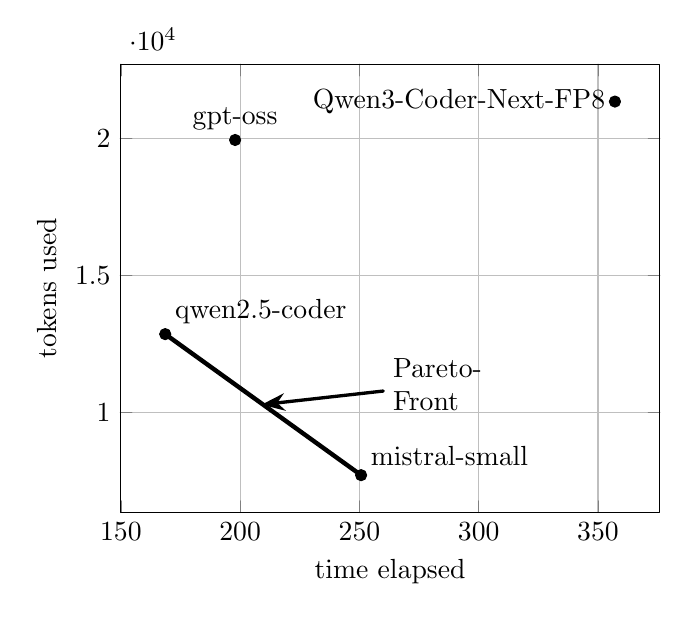
\begin{tikzpicture}[
    >=Stealth,
    line cap=round,
    line join=round,
    node distance=0.2cm
  ]
    \begin{axis}[
        xlabel={time elapsed},
        ylabel={tokens used},
        grid=major
    ]
    \addplot[
        only marks,
        mark=*
    ]   coordinates {
        (197.9, 19951)
        (250.7, 7698)
        (168.6, 12854)
        (357.1, 21356)
    };
    \node[above] at (axis cs:197.9, 19951) {gpt-oss};
    \node[above right] at (axis cs:250.7, 7698) {mistral-small};
    \node[above right] at (axis cs:168.6, 12854) {qwen2.5-coder};
    \node[left] at (axis cs:357.1, 21356) {Qwen3-Coder-Next-FP8};

    \node[anchor=west,text width=3.3em,align=left] (PF) at (axis cs:260,11000) {Pareto-Front};
    
    \draw[->,very thick] (PF) -- (axis cs:209, 10276);
    \draw[ultra thick] (axis cs:168.6, 12854) to (axis cs:250.7, 7698);

    \end{axis}

    
  \end{tikzpicture}
\end{document}
